% Gabarit pandoc des corrigés publiés (brut et guidé). Contenu sans marque ni nom de site.
% Compilation : lualatex (latexmk -lualatex).
% Le Markdown reste la source unique : ne pas éditer ce fichier .tex à la main.
\documentclass[11pt,a4paper]{article}

% --- Moteur, polices (Latin Modern) et langue ---------------------------------
\usepackage{iftex}
\ifLuaTeX\else\errmessage{Ce document se compile avec lualatex}\fi
\usepackage{amsmath,amssymb,mathtools}
\usepackage{fontspec}
% mathrm=sym : \mathrm prend ses glyphes dans la police mathématique (ℓ, μ, Ω), comme KaTeX.
\usepackage[math-style=TeX,bold-style=TeX,mathrm=sym]{unicode-math}
% Repli pour les glyphes absents de Latin Modern (indices et exposants Unicode,
% flèches, filets des schémas en texte, symboles) : DejaVu, puis Latin Modern Math
% (ℓ, lettres mathématiques Unicode des légendes).
\directlua{
  luaotfload.add_fallback("repliTexte", {"DejaVuSerif:mode=harf;", "DejaVuSans:mode=harf;", "file:latinmodern-math.otf:mode=harf;"})
  luaotfload.add_fallback("repliMono", {"DejaVuSansMono:mode=harf;", "DejaVuSans:mode=harf;", "file:latinmodern-math.otf:mode=harf;"})
}
\setmainfont{Latin Modern Roman}[RawFeature={fallback=repliTexte}]
\setsansfont{Latin Modern Sans}[RawFeature={fallback=repliTexte}]
\setmonofont{Latin Modern Mono}[RawFeature={fallback=repliMono}]
\setmathfont{Latin Modern Math}
\usepackage[french]{babel}
\frenchsetup{SmallCapsFigTabCaptions=false}

% --- Mise en page --------------------------------------------------------------
\usepackage[a4paper,margin=2.2cm,headheight=14pt,footskip=1.2cm]{geometry}
\usepackage{microtype}
\setlength{\emergencystretch}{4em}
\tolerance=1500
\setlength{\parindent}{0pt}
\setlength{\parskip}{0.55\baselineskip plus 2pt minus 1pt}
\usepackage{xcolor}
% Gris nommés : babel-french rend « ! » actif dans le document.
\definecolor{gris2}{gray}{0.98}
\definecolor{gris3}{gray}{0.97}
\definecolor{gris5}{gray}{0.95}
\definecolor{gris35}{gray}{0.65}
\definecolor{gris40}{gray}{0.60}
\definecolor{gris45}{gray}{0.55}
\definecolor{gris50}{gray}{0.50}
\definecolor{gris55}{gray}{0.45}
\definecolor{gris60}{gray}{0.40}
\definecolor{gris65}{gray}{0.35}
\definecolor{gris70}{gray}{0.30}
\definecolor{gris80}{gray}{0.20}
\definecolor{gris85}{gray}{0.15}
\usepackage{graphicx}
\usepackage{float}
\usepackage{caption}
\captionsetup{font=small,labelformat=empty,justification=centering}
\usepackage{booktabs,longtable,array,multirow,calc}
\usepackage{siunitx}
\sisetup{locale=FR}
\usepackage[version=4]{mhchem}
\usepackage{listings}
\usepackage{fancyhdr}
\usepackage{lastpage}
\usepackage[most]{tcolorbox}
\usepackage{enumitem}
\setlist{nosep,leftmargin=*,topsep=2pt}
\usepackage[hidelinks,unicode]{hyperref}
\usepackage{bookmark}
\hypersetup{pdftitle={Mines-Ponts MPI — Maths 1 2026},pdfauthor={Rédigé par IA},pdfcreator={LaTeX},pdfsubject={Corrigé brut}}
\usepackage{xurl}

% --- Pandoc : listes, tableaux, figures ----------------------------------------
\providecommand{\passthrough}[1]{#1}
\providecommand{\tightlist}{\setlength{\itemsep}{0pt}\setlength{\parskip}{0pt}}

\makeatletter
\def\maxwidth{\ifdim\Gin@nat@width>\linewidth\linewidth\else\Gin@nat@width\fi}
\def\maxheight{\ifdim\Gin@nat@height>0.55\textheight 0.55\textheight\else\Gin@nat@height\fi}
\makeatother
\setkeys{Gin}{width=\maxwidth,height=\maxheight,keepaspectratio}
\setcounter{secnumdepth}{-\maxdimen}
\providecommand{\pandocbounded}[1]{#1}

% --- Code (listings) -----------------------------------------------------------
\lstset{
  basicstyle=\ttfamily\small,
  columns=fullflexible,
  keepspaces=true,
  breaklines=true,
  breakatwhitespace=false,
  postbreak=\mbox{\textcolor{gris50}{$\hookrightarrow$}\space},
  frame=single,
  rulecolor=\color{gris35},
  framesep=4pt,
  xleftmargin=5pt,xrightmargin=5pt,
  backgroundcolor=\color{gris3},
  keywordstyle=\bfseries,
  commentstyle=\color{gris65},
  stringstyle=\color{gris80},
  showstringspaces=false,
  tabsize=4,
  extendedchars=true,
  aboveskip=6pt,belowskip=6pt,
}

% --- Macros des corrigés (KaTeX ↔ LaTeX) ---------------------------------------
% Les corrigés sont écrits pour KaTeX : on définit ici ce que KaTeX connaît et
% que LaTeX n'a pas, sans jamais retoucher le Markdown.
\providecommand{\R}{\mathbb{R}}
\providecommand{\N}{\mathbb{N}}
\providecommand{\Z}{\mathbb{Z}}
\providecommand{\Q}{\mathbb{Q}}
\providecommand{\C}{\mathbb{C}}
\providecommand{\dd}{\mathrm{d}}
\providecommand{\llbracket}{\lBrack}
\providecommand{\rrbracket}{\rBrack}
\providecommand{\lBrace}{\lbrace}
\providecommand{\rBrace}{\rbrace}
\providecommand{\Box}{\square}
\providecommand{\Diamond}{\lozenge}
\providecommand{\varnothing}{\emptyset}
\providecommand{\argmax}{\operatorname*{arg\,max}}
\providecommand{\argmin}{\operatorname*{arg\,min}}
\renewcommand{\leq}{\leqslant}
\renewcommand{\geq}{\geqslant}

% Équation hors texte : réduite à la largeur de la ligne si elle déborde.
\newsavebox{\boiteequation}
\newcommand{\equationajustee}[1]{%
  \sbox{\boiteequation}{$\displaystyle #1$}%
  \ifdim\wd\boiteequation>\linewidth
    \[\resizebox{\linewidth}{!}{\usebox{\boiteequation}}\]%
  \else
    \[#1\]%
  \fi}

% --- Encadrés pédagogiques (sobres, lisibles en noir et blanc) -----------------
\tcbset{
  encadre/.style={
    enhanced,breakable,sharp corners,
    colback=white,colframe=gris55,
    boxrule=0.4pt,leftrule=2.2pt,
    left=6pt,right=6pt,top=3pt,bottom=3pt,
    before skip=6pt,after skip=6pt,
    fonttitle=\bfseries\small,coltitle=black,
    attach title to upper,after title={\quad},
    parbox=false,
  }
}
\newtcolorbox{indication}[1]{encadre,colframe=gris45,colback=gris2,title={Indication~#1}}
\newtcolorbox{methode}{encadre,colframe=gris70,title={Méthode}}
\newtcolorbox{piege}{encadre,colframe=gris85,boxrule=0.8pt,leftrule=2.2pt,title={Piège}}
\newtcolorbox{jury}{encadre,colframe=gris60,colback=gris5,title={Jury}}
\newtcolorbox{encadrenote}{encadre,colframe=gris40}

% --- Titres de section ---------------------------------------------------------
\usepackage{titlesec}
\titleformat{\section}{\Large\bfseries}{}{0pt}{}
\titleformat{\subsection}{\large\bfseries}{}{0pt}{}
\titleformat{\subsubsection}{\normalsize\bfseries}{}{0pt}{}
\titlespacing*{\section}{0pt}{14pt plus 4pt minus 2pt}{6pt}
\titlespacing*{\subsection}{0pt}{10pt plus 3pt minus 2pt}{4pt}
\titlespacing*{\subsubsection}{0pt}{8pt plus 2pt minus 2pt}{2pt}

% --- En-tête et pied de page ---------------------------------------------------
\pagestyle{fancy}
\fancyhf{}
\fancyhead[L]{\small\textsc{Corrigé brut} · Mines-Ponts MPI}
\fancyhead[R]{\small Maths 1 2026}
\fancyfoot[L]{\footnotesize Corrigé rédigé par IA, non officiel}
\fancyfoot[R]{\footnotesize \thepage\,/\,\pageref*{LastPage}}
\renewcommand{\headrulewidth}{0.4pt}
\renewcommand{\footrulewidth}{0pt}
\fancypagestyle{plain}{\fancyhf{}\fancyfoot[R]{\footnotesize \thepage\,/\,\pageref*{LastPage}}\fancyfoot[L]{\footnotesize Corrigé rédigé par IA, non officiel}\renewcommand{\headrulewidth}{0pt}}

\begin{document}
\thispagestyle{plain}
\begin{center}
  {\small\scshape Corrigé brut}\par\smallskip
  {\LARGE\bfseries Mines-Ponts MPI — Maths 1 2026\par}\medskip
  {\large Mines-Ponts · MPI · Maths 1 · 2026\par}
\end{center}
\vspace{2pt}\hrule\vspace{8pt}

\emph{Corrigé rédigé par IA, non officiel. Signalez toute erreur.}

\textbf{Équation d'Euler-Lagrange et quelques applications.} Durée 3 h, calculatrice interdite.

\hypertarget{i---lemme-fondamental-du-calcul-variationnel}{%
\section{I - Lemme fondamental du calcul variationnel}\label{i---lemme-fondamental-du-calcul-variationnel}}

\hypertarget{question-1}{%
\subsection{Question 1}\label{question-1}}

La fonction \(x\mapsto -1/x\) est de classe \(\mathcal C^\infty\) sur \(\mathbb R_+^\star\) et \(\exp\) est de classe \(\mathcal C^\infty\) sur \(\mathbb R\).

Par composition, \(\varphi:x\mapsto e^{-1/x}\) est de classe \(\mathcal C^\infty\) sur \(\mathbb R_+^\star\).

Montrons par récurrence sur \(n\) qu'il existe \(P_n\in\mathbb R[X]\) tel que, pour tout \(x>0\), \(\varphi^{(n)}(x)=P_n(1/x)\,e^{-1/x}\).

\begin{itemize}
\tightlist
\item
  Initialisation : \(P_0=1\) convient.
\item
  Hérédité : supposons \(\varphi^{(n)}(x)=P_n(1/x)e^{-1/x}\) sur \(\mathbb R_+^\star\).
  La dérivée de \(x\mapsto P_n(1/x)\) est \(x\mapsto-\frac1{x^2}P_n'(1/x)\) (dérivée d'une composée).
  Celle de \(x\mapsto e^{-1/x}\) est \(x\mapsto\frac1{x^2}e^{-1/x}\). Par la formule de dérivation d'un produit, pour \(x>0\) :
\end{itemize}

\equationajustee{\begin{aligned}
\varphi^{(n+1)}(x)&=\left(-\frac1{x^2}P_n'\!\left(\frac1x\right)+\frac1{x^2}P_n\!\left(\frac1x\right)\right)e^{-1/x}\\
&=P_{n+1}\!\left(\frac1x\right)e^{-1/x},
\end{aligned}}

avec

\equationajustee{\boxed{\begin{aligned}P_0&=1\\
P_{n+1}&=X^2\,(P_n-P_n').\end{aligned}}}

\(P_{n+1}\) est un polynôme, ce qui achève la récurrence. Par exemple \(P_1=X^2\) et \(P_2=X^4-2X^3\).

\hypertarget{question-2}{%
\subsection{Question 2}\label{question-2}}

\emph{Lemme.} Pour tout \(Q\in\mathbb R[X]\), \(Q(1/x)e^{-1/x}\to0\) quand \(x\to0^+\).

En effet, avec \(u=1/x\to+\infty\), c'est \(Q(u)e^{-u}\to0\) (croissances comparées).

On utilise le théorème de prolongement de la dérivée (ou de la limite de la dérivée), sur un intervalle \(I\) contenant \(0\) :

\begin{itemize}
\tightlist
\item
  hypothèse 1 : \(g\) est continue sur \(I\) et de classe \(\mathcal C^1\) sur \(I\setminus\{0\}\) ;
\item
  hypothèse 2 : \(g'\) admet une limite finie \(\ell\) en \(0\) ;
\item
  conclusion : \(g\) est de classe \(\mathcal C^1\) sur \(I\) et \(g'(0)=\ell\).
\end{itemize}

Montrons par récurrence sur \(n\) la propriété \(\mathcal Q(n)\) :

\begin{itemize}
\tightlist
\item
  \(\varphi\) est de classe \(\mathcal C^n\) sur \(\mathbb R\) ;
\item
  \(\varphi^{(n)}\) est nulle sur \(\mathbb R_-\) ;
\item
  \(\varphi^{(n)}(x)=P_n(1/x)e^{-1/x}\) pour \(x>0\).
\end{itemize}

\emph{Initialisation.} \(\varphi\) est continue sur \(\mathbb R^\star\).

En \(0\), \(\varphi(x)\to0\) à gauche (fonction nulle) et à droite (lemme avec \(Q=1\)), et \(\varphi(0)=0\). Donc \(\mathcal Q(0)\) est vraie.

\emph{Hérédité.} Supposons \(\mathcal Q(n)\) et posons \(g=\varphi^{(n)}\).

\begin{itemize}
\tightlist
\item
  \(g\) est continue sur \(\mathbb R\), puisque \(\varphi\) est de classe \(\mathcal C^n\).
\item
  \(g\) est de classe \(\mathcal C^1\) sur \(\mathbb R^\star\) : elle est nulle sur \(\mathbb R_-^\star\) et, sur \(\mathbb R_+^\star\), de dérivée \(P_{n+1}(1/x)e^{-1/x}\) (question 1).
\item
  \(g'(x)\to0\) quand \(x\to0^-\) (dérivée nulle) et quand \(x\to0^+\) (lemme appliqué à \(P_{n+1}\)).
\end{itemize}

Le théorème de prolongement de la dérivée donne : \(g\) est de classe \(\mathcal C^1\) sur \(\mathbb R\) et \(g'(0)=0\).

Ainsi \(\varphi\) est de classe \(\mathcal C^{n+1}\) sur \(\mathbb R\).

De plus \(\varphi^{(n+1)}=g'\) est nulle sur \(\mathbb R_-\) et vaut \(P_{n+1}(1/x)e^{-1/x}\) pour \(x>0\). D'où \(\mathcal Q(n+1)\).

Ainsi \(\varphi\) est de classe \(\mathcal C^n\) pour tout \(n\).

\textbf{\(\varphi\) est de classe \(\mathcal C^\infty\) sur \(\mathbb R\)}, avec \(\varphi^{(n)}(0)=0\) pour tout \(n\).

\hypertarget{question-3}{%
\subsection{Question 3}\label{question-3}}

Pour \(c<d\), on pose

\equationajustee{\boxed{\psi_{c,d}(x)=\varphi(x-c)\,\varphi(d-x)\qquad(x\in\mathbb R).}}

\begin{itemize}
\tightlist
\item
  Par composition avec des fonctions affines et produit, \(\psi_{c,d}\) est de classe \(\mathcal C^\infty\) sur \(\mathbb R\) (question 2).
\item
  Si \(x\in\,]c,d[\) : \(x-c>0\) et \(d-x>0\), donc \(\psi_{c,d}(x)=e^{-1/(x-c)}e^{-1/(d-x)}>0\).
\item
  Si \(x\le c\) : \(\varphi(x-c)=0\) ; si \(x\ge d\) : \(\varphi(d-x)=0\). Donc \(\psi_{c,d}=0\) sur \(\mathbb R\setminus\,]c,d[\).
\end{itemize}

\hypertarget{question-4}{%
\subsection{Question 4}\label{question-4}}

Raisonnons par l'absurde : soit \(x_0\in[a,b]\) tel que \(f(x_0)\neq0\).

Quitte à changer \(f\) en \(-f\) (les hypothèses sont inchangées), on peut supposer \(f(x_0)>0\).

Par continuité de \(f\) en \(x_0\), il existe \(\delta>0\) tel que \(f>0\) sur \([a,b]\cap[x_0-\delta,x_0+\delta]\).

Posons \(c=\max(a,x_0-\delta)\) et \(d=\min(b,x_0+\delta)\). Alors \(a\le c\le x_0\le d\le b\).

De plus \(c<d\) : si \(x_0<b\), alors \(d>x_0\ge c\) ; si \(x_0=b\), alors \(c<b=d\) car \(a<b\).

Enfin \(f>0\) sur \([c,d]\).

\begin{figure}[H]
\centering
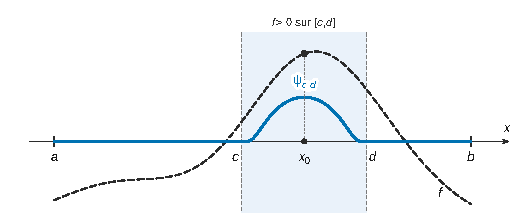
\includegraphics{figures/q4-fonction-plateau.pdf}
\caption*{Figure 1 --- Question 4 : la fonction plateau ψ\_c,d, nulle hors de
l'intervalle ouvert d'extrémités c et d, posée sur un intervalle où f
\textgreater{} 0 (allure de f en tirets)}
\end{figure}

Soit \(h\) la restriction de \(\psi_{c,d}\) à \([a,b]\). Alors \(h\in\mathcal C^\infty([a,b],\mathbb R)\), et \(h(a)=h(b)=0\) car \(a,b\notin\,]c,d[\).

Par hypothèse, \(\int_a^b fh=0\).

Or \(fh\) est continue et positive sur \([a,b]\) : nulle hors de \(]c,d[\), strictement positive sur \(]c,d[\).

Une fonction continue positive d'intégrale nulle sur un segment est nulle. Donc \(fh=0\) sur \([a,b]\), ce qui contredit \((fh)\big(\frac{c+d}2\big)>0\).

\textbf{Donc \(f\) est nulle sur \([a,b]\).}

\emph{Remarque utile pour la suite.} La preuve n'utilise l'hypothèse que pour les fonctions \(h=\psi_{c,d}\) avec \(a\le c<d\le b\). Si \(f(x_0)\neq0\) avec \(x_0\in\,]a,b[\), on peut choisir \(\delta\) assez petit pour que \([c,d]\subset\,]a,b[\).

\hypertarget{ii---uxe9quation-deuler-lagrange}{%
\section{II - Équation d'Euler-Lagrange}\label{ii---uxe9quation-deuler-lagrange}}

\emph{Hypothèse de lecture.} L'énoncé ne suppose \(f\) de classe \(\mathcal C^2\) que sur l'ouvert \(]x_A,x_B[\times U\times V\).

Or les questions 7 à 9 utilisent \(\partial f/\partial y\) et \(\partial f/\partial z\) jusqu'aux bornes \(x_A\) et \(x_B\).

On suppose donc (H) : \textbf{les dérivées partielles de \(f\) d'ordre \(\le2\) se prolongent continûment à \([x_A,x_B]\times U\times V\)}.

C'est le cas dans les trois applications (III, IV, V), où \(f\) ne dépend pas de \(x\) et est de classe \(\mathcal C^\infty\). La lettre \(\varphi\) désigne désormais la fonction définie avant la question 7.

\hypertarget{question-5}{%
\subsection{Question 5}\label{question-5}}

Soit \(y\in\mathcal C\). Comme \(y\) est de classe \(\mathcal C^2\), \(y\) et \(y'\) sont continues.

Donc \(\Gamma:x\mapsto(x,y(x),y'(x))\) est continue sur \([x_A,x_B]\), à valeurs dans \([x_A,x_B]\times U\times V\) par définition de \(\mathcal C\).

Comme \(f\) est continue sur cet ensemble, \(x\mapsto f(x,y(x),y'(x))\) est continue sur le segment \([x_A,x_B]\), donc intégrable sur ce segment : \textbf{\(T(y)\) existe}.

\hypertarget{question-6}{%
\subsection{Question 6}\label{question-6}}

Pour tout \(\varepsilon\), \(y_\varepsilon=z_0+\varepsilon\eta\) est de classe \(\mathcal C^2\).

Comme \(\eta(x_A)=\eta(x_B)=0\), on a \(y_\varepsilon(x_A)=y_0\) et \(y_\varepsilon(x_B)=y_1\).

Il reste à trouver \(\alpha>0\) tel que, pour \(|\varepsilon|<\alpha\) et tout \(x\in[x_A,x_B]\), \(y_\varepsilon(x)\in U\) et \(y_\varepsilon'(x)\in V\).

\begin{figure}[H]
\centering
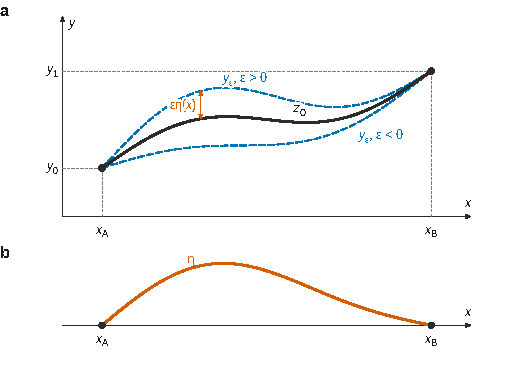
\includegraphics{figures/q6-variation-admissible.pdf}
\caption*{Figure 2 --- Question 6 : perturbations y\_ε = z\_0 + εη de l'extrémale
z\_0, à extrémités fixes ; en bas, la direction η, nulle en x\_A et x\_B}
\end{figure}

Par l'absurde : pour tout \(n\ge1\), il existe \(\varepsilon_n\in\,]-\frac1n,\frac1n[\) et \(x_n\in[x_A,x_B]\) tels que

\equationajustee{z_0(x_n)+\varepsilon_n\eta(x_n)\notin U\quad\text{ou}\quad z_0'(x_n)+\varepsilon_n\eta'(x_n)\notin V.}

L'une des deux éventualités a lieu pour une infinité d'indices ; supposons que ce soit la première.

L'autre se traite de même en remplaçant \((U,z_0,\eta)\) par \((V,z_0',\eta')\), puisque \(z_0'\) et \(\eta'\) sont continues. Quitte à extraire, on suppose la première éventualité vraie pour tout \(n\).

La suite \((x_n)\) est à valeurs dans le segment \([x_A,x_B]\). Par le théorème de Bolzano-Weierstrass, une sous-suite \((x_{\sigma(n)})\) converge vers un \(\ell\in[x_A,x_B]\).

Avec \(M=\|\eta\|_\infty<+\infty\) (\(\eta\) continue sur un segment) :

\equationajustee{\big|z_0(x_{\sigma(n)})+\varepsilon_{\sigma(n)}\eta(x_{\sigma(n)})-z_0(\ell)\big|\le|z_0(x_{\sigma(n)})-z_0(\ell)|+\frac{M}{\sigma(n)}.}

Le membre de droite tend vers \(0\), par continuité de \(z_0\) en \(\ell\).

Or \(z_0(\ell)\in U\) et \(U\) est ouvert : il existe \(r>0\) tel que \(]z_0(\ell)-r,z_0(\ell)+r[\subset U\).

Donc \(z_0(x_{\sigma(n)})+\varepsilon_{\sigma(n)}\eta(x_{\sigma(n)})\in U\) pour \(n\) grand. Contradiction.

\textbf{Il existe donc \(\alpha>0\) tel que \(y_\varepsilon\in\mathcal C\) pour tout \(\varepsilon\in\,]-\alpha,\alpha[\).}

\hypertarget{question-7}{%
\subsection{Question 7}\label{question-7}}

Posons, sur \(]-\alpha,\alpha[\times[x_A,x_B]\),

\equationajustee{g(\varepsilon,x)=f\big(x,z_0(x)+\varepsilon\eta(x),z_0'(x)+\varepsilon\eta'(x)\big),}

de sorte que \(\varphi(\varepsilon)=\int_{x_A}^{x_B}g(\varepsilon,x)\,dx\). Fixons \(\beta\in\,]0,\alpha[\) et travaillons sur \(]-\beta,\beta[\).

\begin{itemize}
\tightlist
\item
  \emph{Régularité en \(\varepsilon\).} Pour \(x\) fixé, \(\varepsilon\mapsto(x,\allowbreak z_0(x)+\varepsilon\eta(x),\allowbreak z_0'(x)+\varepsilon\eta'(x))\) est affine, à valeurs dans \([x_A,x_B]\times U\times V\), où \(f\) est de classe \(\mathcal C^1\) (H).
  Par la règle de la chaîne, \(\varepsilon\mapsto g(\varepsilon,x)\) est de classe \(\mathcal C^1\) et
\end{itemize}

\equationajustee{\frac{\partial g}{\partial\varepsilon}(\varepsilon,x)=\eta(x)\frac{\partial f}{\partial y}\big(x,y_\varepsilon(x),y_\varepsilon'(x)\big)+\eta'(x)\frac{\partial f}{\partial z}\big(x,y_\varepsilon(x),y_\varepsilon'(x)\big).}

\begin{itemize}
\tightlist
\item
  \emph{Continuité en \(x\).} Pour \(\varepsilon\) fixé, \(x\mapsto g(\varepsilon,x)\) et \(x\mapsto\frac{\partial g}{\partial\varepsilon}(\varepsilon,\allowbreak x)\) sont continues sur le segment \([x_A,x_B]\) (composées et produits de fonctions continues).
\item
  \emph{Domination.} L'application \(\Phi:(\varepsilon,\allowbreak x)\mapsto(x,\allowbreak y_\varepsilon(x),\allowbreak y'_\varepsilon(x))\) est continue sur le compact \([-\beta,\beta]\times[x_A,x_B]\).
  Son image \(K\) est donc un compact, inclus dans \([x_A,x_B]\times U\times V\) (question 6).
  Les fonctions \(\partial f/\partial y\) et \(\partial f/\partial z\), continues sur \(K\) par (H), y sont bornées par un réel \(M\).
  D'où, pour \(|\varepsilon|<\beta\) et \(x\in[x_A,x_B]\) :
\end{itemize}

\equationajustee{\left|\frac{\partial g}{\partial\varepsilon}(\varepsilon,x)\right|\le M\big(\|\eta\|_\infty+\|\eta'\|_\infty\big),}

constante indépendante de \(\varepsilon\) et intégrable sur le segment \([x_A,x_B]\).

Le théorème de dérivation des intégrales à paramètre s'applique : \(\varphi\) est de classe \(\mathcal C^1\) sur \(]-\beta,\beta[\) pour tout \(\beta<\alpha\), donc sur \(]-\alpha,\alpha[\), et

\equationajustee{\boxed{\varphi'(\varepsilon)=\int_{x_A}^{x_B}\left(\eta(x)\frac{\partial f}{\partial y}\big(x,y_\varepsilon(x),y_\varepsilon'(x)\big)+\eta'(x)\frac{\partial f}{\partial z}\big(x,y_\varepsilon(x),y_\varepsilon'(x)\big)\right)dx.}}

\hypertarget{question-8}{%
\subsection{Question 8}\label{question-8}}

\emph{\(\varphi'(0)=0\).} Supposons que \(T\) ait un minimum local en \(z_0\) (le cas du maximum est identique).

Il existe \(r>0\) tel que \(T(y)\ge T(z_0)\) pour tout \(y\in\mathcal C\) vérifiant \(\|y-z_0\|_\infty\le r\).

Posons \(\alpha_0=\min\big(\frac\alpha2,\allowbreak \frac{r}{1+\|\eta\|_\infty}\big)\). Pour \(|\varepsilon|\le\alpha_0\), on a \(y_\varepsilon\in\mathcal C\) et

\equationajustee{\|y_\varepsilon-z_0\|_\infty=|\varepsilon|\,\|\eta\|_\infty\le r.}

Donc \(\varphi(\varepsilon)=T(y_\varepsilon)\ge T(z_0)=\varphi(0)\).

Ainsi \(\varphi\) admet un extremum local en \(0\), point intérieur de l'intervalle ouvert \(]-\alpha,\alpha[\), où elle est dérivable. En un extremum local d'une fonction dérivable sur un intervalle ouvert, la dérivée s'annule : \(\varphi'(0)=0\).

Comme \(y_\varepsilon=z_0\) pour \(\varepsilon=0\), la question 7 donne

\equationajustee{\int_{x_A}^{x_B}\left(\eta\,\frac{\partial f}{\partial y}(x,z_0,z_0')+\eta'\,\frac{\partial f}{\partial z}(x,z_0,z_0')\right)dx=0.\qquad(1)}

\emph{Intégration par parties.} Posons \(G(x)=\frac{\partial f}{\partial z}(x,z_0(x),z_0'(x))\).

Comme \(z_0\) est \(\mathcal C^2\), \(x\mapsto(x,z_0(x),z_0'(x))\) est de classe \(\mathcal C^1\).

Comme \(\partial f/\partial z\) est de classe \(\mathcal C^1\) (H), \(G\) est de classe \(\mathcal C^1\) sur \([x_A,x_B]\).

\(\eta\) est de classe \(\mathcal C^1\) et \(\eta(x_A)=\eta(x_B)=0\). Une intégration par parties donne

\equationajustee{\begin{aligned}
\int_{x_A}^{x_B}\eta'G&=\big[\eta G\big]_{x_A}^{x_B}-\int_{x_A}^{x_B}\eta G'\\
&=-\int_{x_A}^{x_B}\eta G'.
\end{aligned}}

En reportant dans (1) :

\equationajustee{\boxed{\int_{x_A}^{x_B}\left(\frac{\partial f}{\partial y}\big(x,z_0(x),z_0'(x)\big)-\frac{d}{dx}\left(\frac{\partial f}{\partial z}\big(x,z_0(x),z_0'(x)\big)\right)\right)\eta(x)\,dx=0.}}

\hypertarget{question-9}{%
\subsection{Question 9}\label{question-9}}

Posons \(F(x)=\frac{\partial f}{\partial y}(x,z_0(x),z_0'(x))-G'(x)\).

Le premier terme est continu (composée de fonctions continues) et \(G'\) est continue (\(G\) est \(\mathcal C^1\)) : \(F\) est continue sur \([x_A,x_B]\).

Soit \(h\in\mathcal C^\infty([x_A,x_B],\mathbb R)\) avec \(h(x_A)=h(x_B)=0\). Elle est de classe \(\mathcal C^2\) et nulle aux bornes : c'est un choix licite de \(\eta\).

Le \(\alpha\) de la question 6 dépend de \(\eta\), mais la conclusion de la question 8 n'en dépend pas. La question 8 donne donc \(\int_{x_A}^{x_B}F h=0\).

Les hypothèses de la question 4 sont vérifiées par \(F\) sur \([a,b]=[x_A,x_B]\) : \(F\) est continue, et son intégrale contre toute \(h\) de classe \(\mathcal C^\infty\) nulle aux bornes est nulle. La question 4 donne \(F=0\) :

\equationajustee{\boxed{\forall x\in[x_A,x_B],\quad \frac{\partial f}{\partial y}\big(x,z_0(x),z_0'(x)\big)-\frac{d}{dx}\left(\frac{\partial f}{\partial z}\big(x,z_0(x),z_0'(x)\big)\right)=0.}}

\emph{Sans l'hypothèse (H)}, on prend seulement \(\eta=\psi_{c,d}\) avec \([c,d]\subset\,]x_A,x_B[\). Ces fonctions sont nulles au voisinage des bornes, et tous les calculs ci-dessus ne font alors intervenir que des points de \(]x_A,x_B[\). La remarque finale de la question 4 donne encore l'équation sur l'ouvert \(]x_A,x_B[\).

\hypertarget{question-10}{%
\subsection{Question 10}\label{question-10}}

Supposons \(\frac{\partial f}{\partial x}=0\) sur \(]x_A,x_B[\times U\times V\) et posons, pour \(x\in\,]x_A,x_B[\),

\equationajustee{B(x)=f\big(x,z_0(x),z_0'(x)\big)-z_0'(x)\,G(x).}

\(f\) est de classe \(\mathcal C^1\) sur l'ouvert et \(x\mapsto(x,z_0(x),z_0'(x))\) est de classe \(\mathcal C^1\), donc \(B\) est de classe \(\mathcal C^1\).

Par la règle de la chaîne, les dérivées partielles étant prises en \((x,z_0(x),z_0'(x))\) :

\equationajustee{\begin{aligned}
B'(x)&=\underbrace{\frac{\partial f}{\partial x}}_{=0}+z_0'\frac{\partial f}{\partial y}+z_0''\frac{\partial f}{\partial z}-z_0''G-z_0'G'\\
&=z_0'(x)\left(\frac{\partial f}{\partial y}\big(x,z_0,z_0'\big)-G'(x)\right)\\
&=0
\end{aligned}}

par l'équation d'Euler-Lagrange (question 9), les termes en \(z_0''\) se compensant car \(G=\partial f/\partial z\).

\(B\) est de dérivée nulle sur l'intervalle \(]x_A,x_B[\), donc constante :

\equationajustee{\boxed{\exists C\in\mathbb R,\ \forall x\in\,]x_A,x_B[,\quad f\big(x,z_0(x),z_0'(x)\big)-z_0'(x)\frac{\partial f}{\partial z}\big(x,z_0(x),z_0'(x)\big)=C.}}

Si \(f\) et \(\partial f/\partial z\) sont continues jusqu'au bord, \(B\) est continue sur \([x_A,x_B]\) et l'égalité vaut aussi en \(x_A\) et \(x_B\).

\hypertarget{iii---le-chemin-le-plus-court-est-la-ligne-droite}{%
\section{III - Le chemin le plus court est la ligne droite !}\label{iii---le-chemin-le-plus-court-est-la-ligne-droite}}

\hypertarget{question-11}{%
\subsection{Question 11}\label{question-11}}

\emph{Vérification des hypothèses de la partie II.} On prend \(U=V=\mathbb R\) (ouverts non vides) et, comme valeurs imposées aux bornes (notées \(y_0\), \(y_1\) en partie II), \(y_A\) et \(y_B\). L'ensemble \(\mathcal C\) de la partie III est alors exactement celui de la partie II.

On définit

\equationajustee{f:[x_A,x_B]\times\mathbb R\times\mathbb R\to\mathbb R,\qquad f(x,y,z)=\sqrt{1+z^2}.}

Comme \(1+z^2>0\), \(f\) est continue et de classe \(\mathcal C^\infty\) (donc \(\mathcal C^2\), et (H) est vraie), et \(T(y)=\int_{x_A}^{x_B}f(x,y(x),y'(x))\,dx\).

\(f\) ne dépend pas de \(x\), donc \(\frac{\partial f}{\partial x}=0\) sur \(]x_A,x_B[\times\mathbb R\times\mathbb R\). Un extremum est en particulier un extremum local : la question 10 s'applique en \(z_0=y_0\).

\emph{Calcul.} On a \(\frac{\partial f}{\partial z}(x,y,z)=\frac{z}{\sqrt{1+z^2}}\), d'où

\equationajustee{\begin{aligned}
f-z\frac{\partial f}{\partial z}&=\sqrt{1+z^2}-\frac{z^2}{\sqrt{1+z^2}}\\
&=\frac1{\sqrt{1+z^2}}.
\end{aligned}}

L'identité de Beltrami donne un réel \(C\) tel que, pour tout \(x\in\,]x_A,x_B[\),

\equationajustee{\frac1{\sqrt{1+y_0'(x)^2}}=C.}

Le membre de gauche appartient à \(]0,1]\), donc \(C\in\,]0,1]\) et \(C\neq0\). On en déduit, sur \(]x_A,x_B[\),

\equationajustee{y_0'(x)^2=\frac1{C^2}-1.}

On note \(k=\sqrt{C^{-2}-1}\ge0\), de sorte que \(y_0'^2=k^2\) sur \(]x_A,x_B[\).

\emph{Résolution.} Ainsi \(y_0'\) est à valeurs dans \(\{-k,k\}\) sur \(]x_A,x_B[\).

Comme \(y_0'\) est continue sur l'intervalle \(]x_A,x_B[\), son image est un intervalle (théorème des valeurs intermédiaires) contenu dans \(\{-k,k\}\) : c'est un singleton.

\(y_0'\) est donc constante sur \(]x_A,x_B[\), puis sur \([x_A,x_B]\) par continuité. \textbf{\(y_0\) est affine}, et les conditions aux bords imposent

\equationajustee{\boxed{y_0(x)=y_A+\frac{y_B-y_A}{x_B-x_A}\,(x-x_A).}}

Le graphe de \(y_0\) est le segment \([AB]\).

\hypertarget{iv---le-chemin-le-plus-rapide-est-la-cyclouxefde}{%
\section{IV - Le chemin le plus rapide est la cycloïde}\label{iv---le-chemin-le-plus-rapide-est-la-cyclouxefde}}

\hypertarget{question-12}{%
\subsection{Question 12}\label{question-12}}

\emph{Lagrangien.} On prend \(U=\mathbb R_+^\star\), \(V=\mathbb R\) et

\equationajustee{f:[x_A,x_B]\times U\times V\to\mathbb R,\qquad f(x,y,z)=\sqrt{\frac{1+z^2}{y}}.}

\(f\) est de classe \(\mathcal C^\infty\) (car \(y>0\)), indépendante de \(x\), donc \(\frac{\partial f}{\partial x}=0\). Toutes ses dérivées sont continues sur \([x_A,x_B]\times U\times V\) : (H) est satisfaite.

\emph{Adaptation de l'ensemble admissible.} L'ensemble \(\mathcal C\) de la partie IV impose en plus \(y'<0\) sur \(]x_A,x_B]\), contrainte qui n'est pas de la forme « \(y'\in V\) ». On utilise seulement des perturbations à support intérieur.

Soient \([c,d]\subset\,]x_A,x_B[\) et \(\eta=\psi_{c,d}\) (restreinte à \([x_A,x_B]\)), de classe \(\mathcal C^\infty\), nulle hors de \(]c,d[\).

Les fonctions continues \(y_0\) et \(-y_0'\) sont minorées respectivement sur les segments \([x_A,x_B]\) et \([c,d]\) par des réels \(m_0>0\) et \(m_1>0\). Posons

\equationajustee{\alpha=\min\left(\frac{m_0}{1+\|\eta\|_\infty},\frac{m_1}{1+\|\eta'\|_\infty}\right).}

Pour \(|\varepsilon|<\alpha\), la fonction \(y_\varepsilon=y_0+\varepsilon\eta\) :

\begin{itemize}
\tightlist
\item
  est de classe \(\mathcal C^2\) et a les mêmes valeurs que \(y_0\) aux bornes ;
\item
  vérifie \(y_\varepsilon>0\) sur \([x_A,x_B]\) et \(y_\varepsilon'<0\) sur \([c,d]\) ;
\item
  vérifie \(y'_\varepsilon=y_0'<0\) sur \(]x_A,x_B]\setminus[c,d]\).
\end{itemize}

Donc \(y_\varepsilon\in\mathcal C\), et \(\varphi(\varepsilon)=T(y_\varepsilon)\ge T(y_0)=\varphi(0)\).

Les questions 7 et 8 s'appliquent alors sans changement : elles n'utilisent que \(y_\varepsilon(x)\in U\) et \(y_\varepsilon'(x)\in V=\mathbb R\).

On obtient \(\int_{x_A}^{x_B}F\,\psi_{c,d}=0\), avec \(F\) continue sur \([x_A,x_B]\). La remarque finale de la question 4 donne \(F=0\) sur \(]x_A,x_B[\).

L'équation d'Euler-Lagrange a donc lieu sur \(]x_A,x_B[\), et le calcul de la question 10 donne l'identité de Beltrami sur \(]x_A,x_B[\).

\emph{Calcul.} On a \(\frac{\partial f}{\partial z}=\frac{z}{\sqrt y\sqrt{1+z^2}}\), donc

\equationajustee{\begin{aligned}
f-z\frac{\partial f}{\partial z}&=\frac1{\sqrt y}\left(\sqrt{1+z^2}-\frac{z^2}{\sqrt{1+z^2}}\right)\\
&=\frac1{\sqrt y\,\sqrt{1+z^2}}.
\end{aligned}}

Il existe donc \(C_1\) tel que, sur \(]x_A,x_B[\),

\equationajustee{\frac1{\sqrt{y_0(x)}\sqrt{1+y_0'(x)^2}}=C_1.}

Le membre de gauche est \(>0\), donc \(C_1>0\), et \(y_0(1+y_0'^2)=\frac1{C_1^2}\) sur \(]x_A,x_B[\).

La fonction \(y_0(1+y_0'^2)\) étant continue sur \([x_A,x_B]\), l'égalité s'étend aux bornes :

\equationajustee{\boxed{\exists C>0,\ \forall x\in[x_A,x_B],\quad y_0(x)\big(1+y_0'(x)^2\big)=C.}}

\hypertarget{question-13}{%
\subsection{Question 13}\label{question-13}}

\(\operatorname{cotan}x=\frac{\cos x}{\sin x}\) est définie si et seulement si \(\sin x\neq0\) : \textbf{domaine \(\mathbb R\setminus\pi\mathbb Z\)}.

Sur \(]0,\pi[\), \(\operatorname{cotan}\) est de classe \(\mathcal C^\infty\) et

\equationajustee{\begin{aligned}
\operatorname{cotan}'(x)&=\frac{-\sin^2x-\cos^2x}{\sin^2x}\\
&=-\frac1{\sin^2x}\\
&=-(1+\operatorname{cotan}^2x)<0.
\end{aligned}}

\(\operatorname{cotan}\) est donc continue et strictement décroissante sur l'intervalle \(]0,\pi[\).

En \(0^+\), \(\cos\to1\) et \(\sin\to0^+\), donc \(\operatorname{cotan}x\to+\infty\).

En \(\pi^-\), \(\cos\to-1\) et \(\sin\to0^+\), donc \(\operatorname{cotan}x\to-\infty\).

Par le théorème de la bijection (fonction continue strictement monotone sur un intervalle), \textbf{\(\operatorname{cotan}\) réalise une bijection de \(]0,\pi[\) sur \(\mathbb R\)}. Sa réciproque \(\operatorname{arccotan}:\mathbb R\to\,]0,\pi[\) est continue et strictement décroissante.

Soient \(t\in\mathbb R\) et \(u=\operatorname{arccotan}t\). On a \(\operatorname{cotan}'(u)=-(1+t^2)\neq0\), donc \(\operatorname{arccotan}\) est dérivable en \(t\), de dérivée \(1/\operatorname{cotan}'(u)\) :

\equationajustee{\boxed{\forall t\in\mathbb R,\quad \operatorname{arccotan}'(t)=-\frac1{1+t^2}.}}

Elle est même de classe \(\mathcal C^\infty\).

On note aussi, pour \(u=\operatorname{arccotan}t\) :

\equationajustee{\sin^2u=\frac1{1+\operatorname{cotan}^2u}=\frac1{1+t^2}.}

\hypertarget{question-14}{%
\subsection{Question 14}\label{question-14}}

Avec \(C=2\), on a \(y_0(x)=\frac2{1+y_0'(x)^2}\).

Posons \(u(x)=\operatorname{arccotan}(y_0'(x))\in\,]0,\pi[\), de sorte que \(\theta(x)=2u(x)\) et \(\operatorname{cotan}u(x)=y_0'(x)\).

Alors \(\sin^2u(x)=\frac1{1+y_0'(x)^2}\) (question 13), et la formule de duplication donne

\equationajustee{\begin{aligned}
y_0(x)&=2\sin^2\frac{\theta(x)}2\\
&=1-\cos\theta(x).
\end{aligned}}

\equationajustee{\boxed{\forall x\in[x_A,x_B],\quad y_0(x)=1-\cos\theta(x).}}

Pour \(x\in\,]x_A,x_B]\), \(y_0'(x)<0\) impose \(u(x)\in\,]\frac\pi2,\pi[\), donc \(\theta(x)\in\,]\pi,2\pi[\).

\hypertarget{question-15}{%
\subsection{Question 15}\label{question-15}}

\(y_0'\) est de classe \(\mathcal C^1\) et \(\operatorname{arccotan}\) de classe \(\mathcal C^\infty\) : \(\theta\) est de classe \(\mathcal C^1\) et

\equationajustee{\begin{aligned}
\theta'(x)&=2y_0''(x)\operatorname{arccotan}'(y_0'(x))\\
&=-\frac{2y_0''(x)}{1+y_0'(x)^2}.
\end{aligned}}

En dérivant \(y_0(1+y_0'^2)=2\) :

\equationajustee{y_0'\big(1+y_0'^2+2y_0y_0''\big)=0.}

Sur \(]x_A,x_B]\), \(y_0'\neq0\), donc \(2y_0y_0''=-(1+y_0'^2)\). Comme \(y_0>0\),

\equationajustee{\theta'(x)=\frac1{y_0(x)}\qquad(x\in\,]x_A,x_B]).}

Posons \(\Lambda(x)=\theta(x)-\sin\theta(x)-x\), de classe \(\mathcal C^1\) sur \([x_A,x_B]\). Pour \(x\in\,]x_A,x_B]\), avec la question 14 :

\equationajustee{\begin{aligned}
\Lambda'(x)&=\theta'(x)\big(1-\cos\theta(x)\big)-1\\
&=\theta'(x)y_0(x)-1\\
&=0.
\end{aligned}}

\(\Lambda\) est constante sur l'intervalle \(]x_A,x_B]\), donc sur \([x_A,x_B]\) par continuité. En notant \(-c\) cette constante :

\equationajustee{\boxed{\exists c\in\mathbb R,\ \forall x\in[x_A,x_B],\quad x=\theta(x)-\sin\theta(x)+c.}}

La courbe \(y_0\) est donc la portion \(\theta\in[\theta(x_A),\theta(x_B)]\subset[\pi,2\pi[\) de la cycloïde \(\theta\mapsto(\theta-\sin\theta+c,\,1-\cos\theta)\). Le cas \(\theta(x_A)=\pi\) correspond à \(y_0'(x_A)=0\).

\begin{figure}[H]
\centering
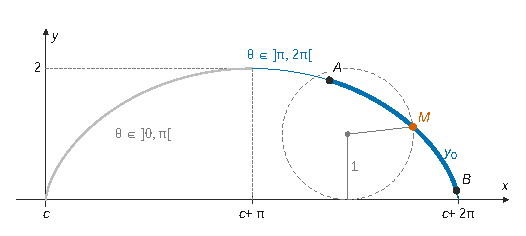
\includegraphics{figures/q15-cycloide.pdf}
\caption*{Figure 3 --- Question 15 : cycloïde décrite par un point M d'une roue de
rayon 1 ; y\_0 est une portion, de A à B, de la branche descendante, où
θ est compris entre π et 2π}
\end{figure}

\emph{Remarque.} Le temps de parcours vaut \(\int ds/v\) avec \(v=\sqrt{2g\,h}\), où \(h\) est la dénivellation depuis le départ.

Le lagrangien \(\sqrt{(1+y'^2)/y}\) suppose donc \(y\) mesuré vers le bas à partir du niveau de \(A\), d'où \(y(x_A)=0\) et \(y\) croissant.

Les conventions de l'énoncé (\(y_A>0\), \(y'<0\)) ne sont pas celles-là ; on a traité le problème comme un problème variationnel.

\hypertarget{v---une-application-uxe0-une-structure-optimale-la-catuxe9nouxefde}{%
\section{V - Une application à une structure optimale : la caténoïde}\label{v---une-application-uxe0-une-structure-optimale-la-catuxe9nouxefde}}

\hypertarget{question-16}{%
\subsection{Question 16}\label{question-16}}

\emph{Vérification des hypothèses de la partie II.} On prend \(x_A=0\), \(x_B=1\), \(U=V=\mathbb R\), et les valeurs imposées aux bornes valent \(1\). L'ensemble \(\mathcal C\) de la partie V est alors celui de la partie II. On définit

\equationajustee{f:[0,1]\times\mathbb R\times\mathbb R\to\mathbb R,\qquad f(x,y,z)=2\pi y\sqrt{1+z^2}.}

\(f\) est continue et de classe \(\mathcal C^\infty\) (donc (H) est vraie), et indépendante de \(x\) : \(\frac{\partial f}{\partial x}=0\).

La fonction \(y_0\) minimise \(T\) sur \(\mathcal C\), donc \(T\) admet en \(y_0\) un extremum local : la question 10 s'applique en \(z_0=y_0\).

\emph{Calcul.} On a \(\frac{\partial f}{\partial z}=\frac{2\pi yz}{\sqrt{1+z^2}}\) et

\equationajustee{f-z\frac{\partial f}{\partial z}=\frac{2\pi y}{\sqrt{1+z^2}}.}

Beltrami donne un réel \(K\) tel que \(\frac{2\pi y_0(x)}{\sqrt{1+y_0'(x)^2}}=K\) sur \(]0,1[\), puis sur \([0,1]\) par continuité.

Posons \(k=K/2\pi\) : \(y_0=k\sqrt{1+y_0'^2}\) sur \([0,1]\).

\emph{Non-nullité.} En \(x=0\), \(y_0(0)=1\) donne \(k=\frac{1}{\sqrt{1+y_0'(0)^2}}>0\). Avec \(c=1/k\neq0\), en élevant au carré :

\equationajustee{\boxed{\exists c\neq0,\ \forall x\in[0,1],\quad 1+y_0'(x)^2=c^2y_0(x)^2.}}

On note aussi que \(y_0=k\sqrt{1+y_0'^2}>0\) sur \([0,1]\).

\hypertarget{question-17}{%
\subsection{Question 17}\label{question-17}}

\(\operatorname{ch}\) est de classe \(\mathcal C^\infty\) sur \(\mathbb R\) et \(\operatorname{ch}'=\operatorname{sh}\), avec \(\operatorname{sh}x=\frac{e^x-e^{-x}}2>0\) pour \(x>0\).

Donc \(\operatorname{ch}\) est continue sur \(\mathbb R_+\) et strictement croissante sur \(\mathbb R_+\) (dérivée \(>0\) sur \(\mathbb R_+^\star\), continuité en \(0\)).

Comme \(\operatorname{ch}0=1\) et \(\operatorname{ch}x\to+\infty\) en \(+\infty\), le théorème de la bijection donne : \textbf{\(\operatorname{ch}\) réalise une bijection de \(\mathbb R_+\) sur \([1,+\infty[\)}.

Sa réciproque \(\operatorname{argch}:[1,+\infty[\to\mathbb R_+\) est continue et strictement croissante.

Soient \(t>1\) et \(u=\operatorname{argch}t>0\). Alors \(\operatorname{ch}'(u)=\operatorname{sh}u>0\), et \(\operatorname{sh}u=\sqrt{\operatorname{ch}^2u-1}=\sqrt{t^2-1}\) car \(\operatorname{sh}u>0\). Donc

\equationajustee{\boxed{\forall t>1,\quad \operatorname{argch}'(t)=\frac1{\sqrt{t^2-1}}.}}

En \(t=1\), \(\operatorname{ch}'(0)=0\) et \(\operatorname{argch}\) n'est pas dérivable : pour \(u=\operatorname{argch}t\to0^+\),

\equationajustee{\frac{\operatorname{argch}t-\operatorname{argch}1}{t-1}=\frac{u}{\operatorname{ch}u-1}\sim\frac2u,}

qui tend vers \(+\infty\) quand \(t\to1^+\).

\hypertarget{question-18}{%
\subsection{Question 18}\label{question-18}}

Quitte à changer \(c\) en \(-c\), on suppose \(c>0\).

Par hypothèse \(c^2y_0^2>1\), et \(y_0>0\) (question 16), donc \(cy_0(x)>1\). Comme \(y_0'>0\), on a \(y_0'=\sqrt{c^2y_0^2-1}\).

La fonction \(\Psi(x)=\operatorname{argch}(cy_0(x))\) est dérivable, car \(cy_0\) est \(\mathcal C^1\) à valeurs dans \(]1,+\infty[\), et

\equationajustee{\Psi'(x)=\frac{c\,y_0'(x)}{\sqrt{c^2y_0(x)^2-1}}=c.}

Donc \(\Psi(x)=cx+K\) sur \([0,1]\), avec \(K=\operatorname{argch}(c)>0\) (car \(c=cy_0(0)>1\)). En appliquant \(\operatorname{ch}\) :

\equationajustee{\boxed{y_0(x)=\frac1c\operatorname{ch}(cx+K)\qquad(x\in[0,1]),}}

\(K\) étant une constante d'intégration.

Réciproquement, une telle fonction vérifie

\equationajustee{\begin{aligned}
1+y_0'^2&=1+\operatorname{sh}^2(cx+K)\\
&=\operatorname{ch}^2(cx+K)\\
&=c^2y_0^2.
\end{aligned}}

\textbf{Erreur d'énoncé.} L'hypothèse « \(y_0'>0\) sur \([0,1]\) » est incompatible avec \(y_0(0)=y_0(1)=1\) : \(y_0\) serait strictement croissante.

Aucune fonction ne vérifie toutes les hypothèses. Le calcul ci-dessus est ce que la question demande, mais il ne décrit pas le film de savon. Voici la détermination correcte, sans hypothèse de signe.

Le cadre de la partie V étant celui de la partie II (\(U=V=\mathbb R\), (H) vraie), l'équation d'Euler-Lagrange (question 9) s'applique.

On a \(\frac{\partial f}{\partial y}=2\pi\sqrt{1+z^2}\) et \(\frac{\partial f}{\partial z}=\frac{2\pi yz}{\sqrt{1+z^2}}\). Notons \(p=y_0'\) ; alors

\equationajustee{\begin{aligned}
\frac{d}{dx}\left(\frac{y_0p}{\sqrt{1+p^2}}\right)&=\frac{p^2+y_0y_0''}{\sqrt{1+p^2}}-\frac{y_0p^2y_0''}{(1+p^2)^{3/2}}\\
&=\frac{p^2(1+p^2)+y_0y_0''}{(1+p^2)^{3/2}}.
\end{aligned}}

Après division par \(2\pi\), l'équation d'Euler-Lagrange s'écrit

\equationajustee{\sqrt{1+p^2}=\frac{p^2(1+p^2)+y_0y_0''}{(1+p^2)^{3/2}},}

c'est-à-dire \((1+p^2)^2-p^2(1+p^2)=y_0y_0''\). Avec la question 16 :

\equationajustee{\begin{aligned}
y_0\,y_0''&=1+y_0'^2\\
&=c^2y_0^2.
\end{aligned}}

Comme \(y_0>0\), on obtient

\equationajustee{y_0''=c^2y_0.}

C'est une équation linéaire : \(y_0=A\operatorname{ch}(cx)+B\operatorname{sh}(cx)\).

La condition \(y_0(0)=1\) donne \(A=1\), et \(y_0(1)=1\) donne \(B=\frac{1-\operatorname{ch}c}{\operatorname{sh}c}=-\operatorname{th}\frac c2\). Donc

\equationajustee{y_0(x)=\frac{\operatorname{ch}\big(c(x-\frac12)\big)}{\operatorname{ch}(c/2)}.}

Enfin, en \(x=\frac12\), \(y_0'(\frac12)=0\). La relation de la question 16 donne alors \(1=c^2y_0(\frac12)^2=\frac{c^2}{\operatorname{ch}^2(c/2)}\), d'où \(\operatorname{ch}(c/2)=c\) et

\equationajustee{\boxed{\begin{aligned}y_0(x)&=\frac1c\operatorname{ch}\!\left(c\left(x-\frac12\right)\right),\\
\operatorname{ch}\frac c2&=c\quad(c>0).\end{aligned}}}

C'est la forme \(\frac1c\operatorname{ch}(cx+K)\) avec \(K=-\frac c2<0\).

\(y_0'\) s'annule en \(\frac12\) (col de la caténoïde), ce qui confirme l'incompatibilité des hypothèses de l'énoncé.

\emph{Existence de \(c\).} Avec \(u=c/2\), il faut \(\operatorname{ch}u=2u\).

\(G(u)=\operatorname{ch}u-2u\) est strictement convexe (\(G''=\operatorname{ch}>0\)), donc s'annule au plus deux fois.

On a \(G(\frac12)=\operatorname{ch}\frac12-1>0\) et \(G(\ln2)=\frac54-2\ln2<0\), car \(e^5<243<256=2^8\) donne \(\ln2>\frac58\). Enfin \(G\to+\infty\) en \(+\infty\).

Il y a exactement deux solutions, \(u_1\approx0{,}589\) et \(u_2\approx2{,}127\), soit \(c\approx1{,}18\) ou \(c\approx4{,}25\).

On obtient deux caténoïdes, d'aires \(\approx5{,}99\) et \(\approx6{,}85\). Seule la première (col de rayon \(\approx0{,}85\)) peut minimiser l'aire.

\begin{figure}[H]
\centering
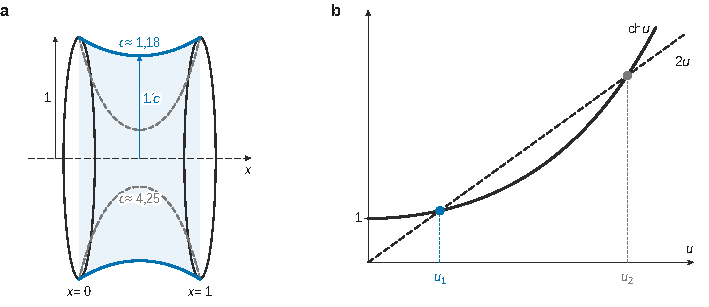
\includegraphics{figures/q18-catenoide.pdf}
\caption*{Figure 4 --- Question 18 : (a) les deux caténoïdes s'appuyant sur les
cercles x = 0 et x = 1, col de rayon 1/c ; (b) leurs constantes c = 2u
viennent des deux racines de ch u = 2u}
\end{figure}

\end{document}
